\documentclass[10pt,a4paper,final,oneside,openany,article,twocolumn]{memoir}
% [12pt, 11pt, landscape, titlepage, a4paper, draft, twoside, oneside, 
%  openleft, openright, openany]

%\chapterstyle{article}

%BASIC PACKAGES
\usepackage{eso-pic,fix-cm,ae,aecompl,ifthen}         
\usepackage[danish,english]{babel} % last language decides document language!
\usepackage[utf8x]{inputenc}          %text encoding
\usepackage{amsmath,amssymb, amsbsy}  % math
\usepackage{graphicx}
\usepackage[usenames,dvipsnames]{color}
\usepackage[british]{isodate} 
%\usepackage{morefloats}
\usepackage[style=alphabetic,natbib=true]{biblatex}
\usepackage{amsmath}
\usepackage[sc]{mathpazo}
\usepackage{MnSymbol}
\usepackage{booktabs} % nicer spacing between table rulers

\usepackage{fixltx2e} % To prevent the figures from being placed out-of-order with respect to their "non-starred" counterparts

%\bibliographystyle{apalike}
\bibliography{../bibliography}


\newsubfloat{figure}

%MISC. PACKAGES
%\usepackage{multicol}        % \begin{multicols}{2} \end{multicols}
%\usepackage{array}           % advanced tables
%\usepackage{multirow}        % advanced tables
%\usepackage{longtable}       % split tables over pages
%\usepackage{textcomp}        % symbols
%\usepackage{verbatim}        % monospace code environment
%\usepackage{pdflscape}       % \begin{landscape} \end{landscape}
%\usepackage{semantic}        % Good for proof trees and math ligatures
\usepackage[noend]{algorithmic}
\usepackage{algorithm}
\usepackage{microtype}        % AWESOME typography!
%\usepackage{colortbl}
%\usepackage{marvosym}
%Kan bruges som \fixme{blabla}. Vises sålænge tex doc er i draft.
\usepackage[draft]{fixme}


%FONT
\usepackage[T1]{fontenc}
\usepackage{palatino}              % font : garamond
\linespread{1.05}                  % Palatino needs more leading (space between lines)
%\usepackage[scaled]{beramono}
\renewcommand{\ttdefault}{cmtt}    % alternative monospace font
%\renewcommand{\rmdefault}{ugm}
%\usepackage{euler}                % weirdo math
%PAGE DIMENSIONS

%\usepackage[left=4.5cm, right=4.5cm, top=4.4cm, bottom=4.5cm]{geometry}


%HEADERS
\makepagestyle{myheadings}

%\makepsmarks{myheadings}{
%  \def\chaptermark##1{\markboth{%
%    \ifnum \value{secnumdepth} < -1
%      \if@mainmatter
%        \chaptername\ \thechapter\ --- %
%      \fi
%    \fi
%    ##1}{}}

%  \def\sectionmark##1{\markright{%
%    \ifnum \value{secnumdepth} < 0
%      \thesection. \ %
%    \fi
%    ##1}}
%}
%%\makeevenhead{myheadings}{\thechapter\hskip.3cm\vrule\hskip.3cm \leftmark}{}{}
%\makeoddhead{myheadings}{}{}{\leftmark\hskip.3cm\vrule\hskip.3cm\thechapter}
%%\makeoddhead{myheadings}{}{}{\rightmark\hskip.3cm\vrule\hskip.3cm\thesection}
%\makeevenfoot{myheadings}{}{\thepage}{}
%\makeoddfoot{myheadings}{}{\thepage}{}
%\pagestyle{myheadings}

% customize chapter pages

\makepagestyle{myheadingschapterpage}
  \makeevenfoot{myheadingschapterpage}{}{}{\thepage}
  \makeoddfoot{myheadingschapterpage}{}{}{\thepage}
\aliaspagestyle{chapter}{myheadingschapterpage}
\aliaspagestyle{title}{myheadingschapterpage}
\makeevenhead{myheadings}{}{\scshape \thetitle}{}
\makeoddhead{myheadings}{}{\footnotesize\scshape \thetitle}{}
\makeevenfoot{myheadings}{}{}{\thepage}
\makeoddfoot{myheadings}{}{}{\thepage}
\pagestyle{myheadings}



%PDF OUTPUT
\usepackage{hyperref}             % clickable url's in PDF-output
\hypersetup{
%    unicode=true,          % non-Latin characters in Acrobat’s bookmarks
%    pdftitle={My title},    % title
%    pdfauthor={Author},     % author
%    pdfsubject={Subject},   % subject of the document
%    pdfcreator={Creator},   % creator of the document
%    pdfproducer={Producer}, % producer of the document
%    pdfkeywords={keywords}, % list of keywords
%    pdfnewwindow=true,      % links in new window
    colorlinks=true,       % false: boxed links; true: colored links
    linkcolor=black,          % color of internal links
    citecolor=black,        % color of links to bibliography
    filecolor=black,      % color of file links
    urlcolor=black           % color of external links
}




%PRETTY COLORS
\usepackage{color}
\definecolor{blue}{rgb}{0,0,0.8}
\definecolor{green}{rgb}{0,0.5,0}
\definecolor{red}{rgb}{0.5,0,0}
\definecolor{grey}{rgb}{0.5,0.5,0.5}


%SECTION TITLES
\def\thefigure{\arabic{figure}}
%\def\thesection{\arabic{section}}
%\def\thesubsection{\thesection.\arabic{subsection}}
%\def\thesubsubsection{\alph{subsubsection}.}
% \alph \roman \arabin
\setcounter{tocdepth}{0}


% USER DEFINED COMMANDS AND ENVIRONMENTS
%\newcommand{\codevar}[1]{{\tt{\it #1}}}
%\newcommand{\genericleft}{\langle\hspace{-2.6pt}\vert}  % prints [[
%\newcommand{\genericright}{\vert\hspace{-2.6pt}\rangle} % prints ]]
%\newcommand{\generic}[1]{\genericleft #1 \genericright^{\varepsilon}}

%FIGURE CAPTIONS
%\usepackage[labelformat=empty]{subfig}
\usepackage{sidecap} % side captions: \begin{SCfigure}[2.7][ht] ...
\usepackage{caption}
\captionsetup{margin=0pt, font=small, labelfont=bf, format=hang}
\setlength{\abovecaptionskip}{0pt}
\setlength{\belowcaptionskip}{0pt}

%LINE SPACING
%\usepackage{setspace}
%EXAMPLE:
% \singlespacing, \onehalfspacing, \doublespacing, \setstretch{x}


%PROGRAM CODE WITH HIGLIGHTING AND SHAZZ!
%\usepackage{listings}



%DOCUMENT INFO
\title{\vspace{-1.5cm}
  Fitting an All-atom Protein Model to a $C_\alpha$-trace\\
}
\author{
	Martin Dybdal -- \texttt{dybber@dybber.dk}\\
	Anders Boesen Lindbo Larsen -- \texttt{abll@diku.dk} \\
	Esben Skaarup -- \texttt{sben@sben.dk}
}

%\datebritish
\date{16th July 2010}

\newcommand{\subimgwidth}{.48\textwidth}
\newcommand{\imgwidth}{.85\textwidth}
\renewcommand\v[1]{\boldsymbol{#1}}
\newcommand{\Ca}{C$_{\alpha}${}}
\newcommand{\rotateAround}[1]{\lcirclearrowright \hspace{-3mm}\colorbox{white}{}{} \hspace{-1.7mm} _{\scriptscriptstyle #1}}
\setcounter{secnumdepth}{1}
\setcounter{chapter}{0}
%\renewcommand\thesection{\arabic{section}}
\setsecheadstyle{\large\bfseries\raggedright}
\setsubsecheadstyle{\bfseries}

\twocoltocetc
\setlength{\absleftindent}{1.5cm}
\setlength{\absrightindent}{\absleftindent}
			
\begin{document}
\twocolumn[\maketitle
\begin{onecolabstract}
  \vspace{-0.2cm}
  Protein structure prediction can be simplified by using a model
  that only includes a subset of the atoms present in proteins. In
  particular, the algorithms group at our department only predicts a
  folding of the $C_\alpha$-trace, and are thus excluding most
  backbone atoms and all side-chain molecules.

  In this report we investigate a strategy for predicting the native
  structure of proteins including all atoms (an all-atom model), where
  we use an already folded $C_\alpha$-trace as target. The strategy
  divides the problem into two separate tasks.

  The first task is to build the all-atom protein backbone with the
  given $C_\alpha$-trace as target. To solve the inverse kinematics
  problem of adjusting the backbone structure we use cyclic coordinate
  descent on consecutive overlapping windows within the backbone.
  Typically we are able to reach an RMSD less than 0.2 Å.


  The second task is to position side-chains on the backbone and
  selecting side-chain conformations in a way that minimizes the
  number of collisions. We have devised an algorithm that iteratively
  goes through each amino acid eliminating eventual collisions when
  possible. The collision avoidance algorithm is on average reducing
  the number of collisions in proteins by a factor ten.
  \vspace{1.5cm}
\end{onecolabstract}
]
\tableofcontents*

\newpage


\hspace*{1.3cm}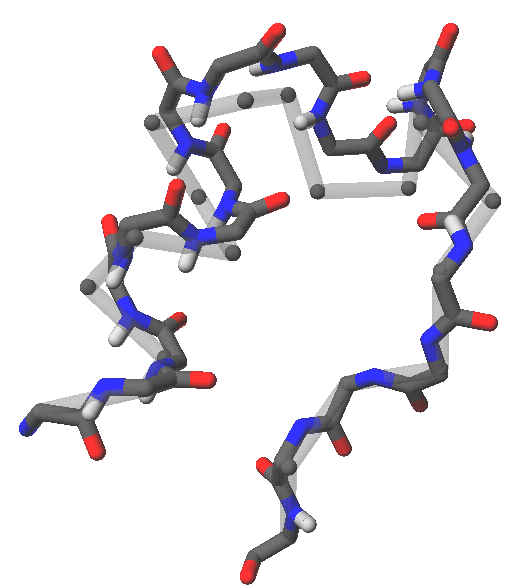
\includegraphics[width=0.4\textwidth]{figures/forside.png}

%\listoffixmes

\newpage
\chapter{Introduction}
\label{chap:intro}
Proteins is the perhaps most important molecules of living
organisms. They perform a multitude of biological tasks and is found
in all lifeforms, from bacteria and unicellular organisms to
multicellular organisms such as animals. The chemical abilities and
biological functions of proteins is determined by their
three-dimensional structure. The ability to determine this structure
without performing costly experiments will have many applications in
medicine (e.g. drug design) and biotechnology. Protein structure
prediction and the related topic protein folding\footnote{The two
  research fields are distinguished by whether the actual folding
  process is simulated (protein folding) or a legal structure is
  sought without computing the intermediate steps (protein structure
  prediction).} are large and active research fields. It is still an
open problem.

\section{Protein structure}
The building blocks of proteins are amino acids\footnote{A detailed
  introduction to the structure of proteins is found in
  \cite{branden}}. There are twenty different amino acids which all
share a common structure. The type of amino acid is identified by an
attached molecule called the side-chain. A protein consists of one or
several unbranched chains (polymers) of amino acids. The order of
amino acids in such a chain is the primary structure of the protein.
The structure diagram in Figure \ref{fig:amino_connect} shows how a
sequence of amino acids are connected. The carbon atom connecting the
backbone with the side-chains is called the $C_\alpha$-atom. It is the
torsional angles around the two bonds connecting $C_\alpha$-atoms with
its neighbours ($N-C_\alpha$ and $C_\alpha-C'$), that contributes with
the highest variability to the determination of the protein structure
(see Section \ref{chap:protein_geometry}). Thus, when solving the
structure prediction problem it is common \fxwarning{cite} to cut down
the problem by using a model that describes the protein solely by its
$C_\alpha$-atoms. Such a sequence of $C_{\alpha}$ atoms is called a
$C_{\alpha}$-trace (see Figure \ref{fig:Calpha_backbone}). This is
also the representation used by the algorithms group at our department
and they therefore requested a method for subsequently adding the
remaining atoms to their model.

In Section \ref{chap:protein_geometry} we will describe the geometry
of the protein backbone and its side chains in detail.

%% Evt. Secondary structure: $\alpha$-helices, $\beta$-sheets
%% (+strands) and loops/turns.


\begin{figure}
  \centering
  \subbottom[]{
    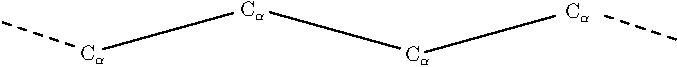
\includegraphics[width=0.48\textwidth]{figures/Calpha_backbone}  
    \label{fig:Calpha_backbone}
  }
  \subbottom[]{
    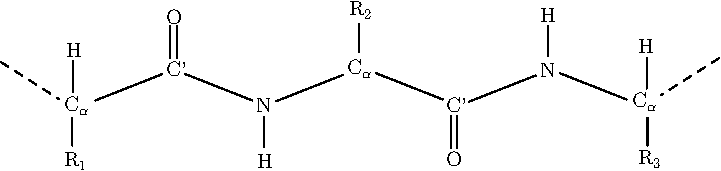
\includegraphics[width=0.48\textwidth]{figures/amino_connect}  
    \label{fig:amino_connect}
  }
  \caption{(a) $C_{\alpha}$-trace. (b) All-atom protein backbone, with $R_1$, $R_2$ and $R_3$ representing side-chains}
\end{figure}

\section{Protein structure prediction}
The chemical stability of a protein molecule is determined by the
amount of free energy in its structure. It is hypothesized
(\textit{Anfinsens dogma} or the \textit{thermodynamic hypothesis},
\cite{anfinsen73, soundararajan2010}) that all proteins has a unique
stable conformation where the free energy is minimized. This
conformation is known as the native structure of the
protein. Determining it computationally is the problem of protein
structure prediction. Thus, protein structure prediction is an energy
minimization problem.

% Why simplifications are necessary to make the problem
% computationally feasible.

There are generally two approaches to protein structure prediction.
\textit{Comparative modelling} uses information from known template
proteins with similar amino acid sequences while performing the
prediction. Another approach, called \textit{ab initio} or
\textit{de novo}, starts ``from scratch'' in the sense that no
information from known structures are used, but instead the
physical/chemical interactions between atoms forms the basis. This
\textit{ab initio} strategy is the approach taken by the algorithms
group at our department.

\subsection{Evaluating predictions}
%http://cnx.org/content/m11608/latest/
To determine the quality of prediction algorithms it is common \fxwarning{cite}
to compare predicted structures of a test proteins with the actual
known structure of that protein. The known structure of such test
proteins are obtained by other means (e.g. X-ray crystallography).
Thus a comparison measure between protein conformations are
needed. The most widely used comparison measure is \textit{least root mean
  square deviation}, lRMSD. RMSD is based on the distances between
corresponding atoms in the two protein conformations under comparison.
If $\vec{A}$ and $\vec{B}$ are two different conformations of the same protein,
where $\vec{a}_i$ and $\vec{b}_i$ are the respective coordinates of atom $i$ in the two
structures, RMSD can be computed by:
\begin{equation}
  \label{eq:rmsd}
  D(\vec{A}, \vec{B}) = \sqrt{\frac{1}{n}\sum_{i=1}^n |\vec{a}_i - \vec{b}_i|^2}
\end{equation}
To compute lRMSD, the RMSD has to be minimized by rotation and
translation of the two conformations. That is, to compute lRMSD, an
\textit{optimal superpositioning} of the conformations is found and
RMSD is computed.


% Limitation: A realistic energy calculation will require an insight in biochemistry
% that is beyond the scope of this project.  Therefore, we limit
% ourselves to minimize the number of clashes as well as the deviation
% from the provided $C_\alpha$-trace.


\section{Our strategy}
As mentioned, the algorithms group at our department uses a model that
only includes the the $C_\alpha$-atoms. Our goal with this project is
to extend this model with the remaining atoms to get an all-atom
model.  This will also enable the algorithms group to participate in
the CASP experiment \cite{caspwebsite}.

The strategy we will pursue, is to use a given $C_\alpha$-trace
generated by their prediction algorithm as target when fitting a
protein model that contains all atoms. The fitting should be conducted,
such that it minimizes the number of clashes and at the same time
minimizes the deviation from the target $C_\alpha$-trace.

We consider our fitting problem as two somewhat separate problems.
First, the backbone must be fitted to the \Ca-trace, only minimizing
the deviation to the $C_{\alpha}$-trace.  Hereafter, the amino acid
residues (side chains) are added to the backbone changing the backbone
conformation only if necessary.  In the following we have chosen to
consider these two tasks separately even though the residue handling
will cause changes in the backbone.

In Section \ref{chap:fitting_backbone}, we will describe the strategy we use to fit the all-atom backbone to the \Ca-trace ignoring the amino acid residues.
In Section \ref{chap:handling_sidechains}, we will explain how we add the side-chains to the all-atom backbone changing the backbone-conformation only if necessary.

%By considering these tasks separately, we simplify our solution since ... \fixme{begrund hvorfor}
%Fitting the backbone while taking side-chain placement into consideration 
%%Her vil vi gå igennem vores overordnede strategi:


\chapter{Protein geometry}
\label{chap:protein_geometry}
The representation of proteins shown in the structure diagram of
Figure \ref{fig:amino_connect} is suitable for determining the
chemical properties of the molecules, getting an overview of how atoms
are arranged and how the atoms are connected. However, to get an exact
model of the protein structure we need a lot more precision in our
characterization. That is, we need to include the concepts of bond
lengths, bond angles and torsional angles into the model.  We suggest
that you refer to Figure \ref{fig:protein-torsion-angles} while
reading the following explanation the concepts.

\subsection{Dataset}
To obtain suitable values we have run statistics on a collection of
proteins from \url{pdb.org}. We downloaded a set of around 730 protein
descriptions (randomly chosen from the site) and removed proteins with
unrealistic bond lengths (as we assume that these proteins descriptors
contained errors). Our final data set consists of 645 proteins.


\section{Backbone geometry}
\textit{Bond lengths} are the distances between the individual atoms
in a molecule (usually measured in Ångstrøm). We will name the
individual bond lengths by the name of the two atoms which the bond
connects, e.g. the bond between a \Ca\ and N atom in an amino acid of
the protein backbone is called \Ca -N. We have computed bond lengths
for all bonds in the backbone, the results are shown in Table
\ref{tab:average_bond_lengths}. As can be seen from the last column in
the table, the variation is very constrained and we therefore havenøt
found it necessary to consider making any variations from the mean
lengths. 
%% Actually, these variations are so small that they can very possibly
%% be attributed to uncertainty in the measuring equipment.

\begin{table}
  \centering
  \begin{tabular}{lrr}
    \toprule
    \multicolumn{1}{c}{Bond} & \multicolumn{1}{c}{Avg. length} & \multicolumn{1}{c}{Std.dev.} \\ \midrule 
    C-O   & 1.2260 Å & 0.0188 Å\\
    CA-C  & 1.5272 Å & 0.0191 Å\\
    N-CA  & 1.4680 Å & 0.0237 Å\\
    C-N   & 1.3234 Å & 0.0215 Å\\
    N-H   & 0.9793 Å & 0.0342 Å\\
    CA-CB & 1.5327 Å & 0.0228 Å\\
    CA-HA & 1.0747 Å & 0.0307 Å\\ \bottomrule
  \end{tabular}
  \vspace{1mm}
  \caption{Average bond lengths (in ångstrøm)}
  \label{tab:average_bond_lengths}
\end{table}

A \textit{bond angle} is an angle between two outgoing bonds from a
single atom. As an example, the angle between the bonds N-\Ca\ and \Ca
-C' is called N-\Ca -C'. Table \ref{tab:average_bond_angles} shows
average values for the backbone bond angles in degrees. Again can we
see that the variation is very limited, but as a small angular
displacement can have a rather large influence on the remaining part
of the protein, they could still introduce variability into the model
of much larger order. In this project we have however selected to
focus solely on the variability in the torsional angles, thus locking
the bond angles to their mean values.

\begin{table}
  \centering
  \begin{tabular}{l>{$}r<{^\circ$}>{$}r<{^\circ$}}
    \toprule
    \multicolumn{1}{c}{Bond} & \multicolumn{1}{c}{Avg. angle} & \multicolumn{1}{c}{Std.dev.} \\ \midrule 
    H-N-CA & 118.9553 & 1.9979\\
    N-CA-C & 110.6099 & 2.4668\\
    CA-C-O & 120.7088 & 1.3064\\
    CA-C-N & 116.7804 & 1.7682\\
    C-N-CA & 121.4547 & 1.9946\\
    C-N-H  & 119.5112 & 2.1599\\ \bottomrule
  \end{tabular}
  \vspace{1mm}
  \caption{Average bond angles (in degrees)}
  \label{tab:average_bond_angles}
\end{table}


\begin{figure*}
  \centering
  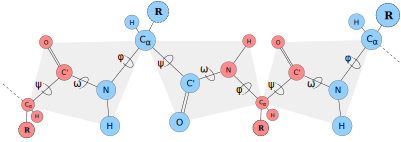
\includegraphics[width=0.75\textwidth]{figures/protein-torsion-angles}
  \caption{Illustration of the protein torsion angles in a protein sequence extract.}
  \label{fig:protein-torsion-angles}
\end{figure*}

A \textit{torsional angle} is rotational angle around a bond. In the
backbone, there are three of such torsional angles (see Figure
\ref{fig:protein-torsion-angles}). The $\phi$ and $\psi$ angles were
mentioned earlier and we will return to them after this paragraph. The
last one, the $\omega$-angle, is almost always $180^{\circ}$
\cite{probik}, but at a few occurrences it deviates from this
value. We will assume that the $\omega$ angle is \textit{always}
$180^{\circ}$. This makes the grey rectangular areas of Figure
\ref{fig:protein-torsion-angles} completely rigid.  Each of the
torsional angles can be defined as dihedral angles between two
planes. For example, the $\phi$ angle can be described by the angle
between the two planes defined by the atoms C'$_{n-1}$, N$_n$ and \Ca
$_n$ as well as N$_n$, \Ca $_n$ and C'$_n$. Thus, four atoms are
needed to define a dihedral angle.

Getting back to the $\phi$ and $\psi$, we can now see that these are
the main variability of the protein backbone, as all bond lengths and
bond angles are nearly rigid and the $\omega$-angle has rarely
deviates from the $180^\circ$ value. 

Because of collisions between side-chains and the backbone, only
certain combinations of $\phi$ and $\psi$ angles are legal. The legal
angles can be illustrated graphically in what is known as a
\textit{Ramachandran plot} (Figure \ref{fig:ramachandran}). In the
plot on the left (Figure \ref{fig:ramachandran}) legal values for all
amino acids except Glycine has been shown. And in the right plot legal
values for Glycine has been shown. Glycine is special because of its
simplicity. It consists of a single H atom connected to the $C_\alpha$
of the amino acid and thus collisions with the backbone is hardly a
problem.

\begin{figure*}
	\centering
	\subbottom[]{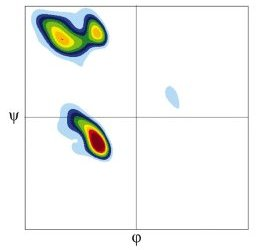
\includegraphics[width=0.3\textwidth]{figures/ramachandran_except_gly} \label{fig:ramachandran}}
    \subbottom[]{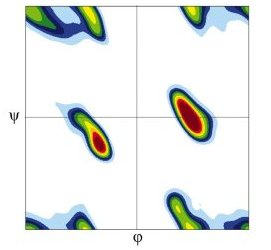
\includegraphics[width=0.3\textwidth]{figures/ramachandran_only_gly} \label{fig:ramachandran_gly}}
    \caption{\textbf{(a)} A ramachandran plot for all amino
      acids except Glycine. \textbf{(b)}  Ramachandran plot
      for Glycine. The figure is from Wikipedia, licensed under Creative Commons.}
\end{figure*}

% \subsection{Additional measurements}
% To place the atoms we have had the need to obtain further measures

\section{Side-chain geometry}
\begin{figure}
	\centering
	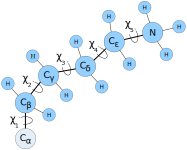
\includegraphics[width=0.35\textwidth]{figures/lysine}
    \caption{Illustration of the $\chi$-angles on the side chain of Lysine (LYS).}
    \label{fig:lysine-and-chi}
\end{figure}
\fixme{Skift til en ordentlig skrifttype på figuren}

As for the backbone, the side chains can be described by bond lengths,
bond angles and a few torsional angles (see below), but to simplify
how we construct the proteins, we have chosen to use another
representation. We store the side chain of each amino acid by the
position of the individual atoms when all torsional angles are zero
and using a coordinate system that has $C_\alpha$ as origo and
orientated such that the $C_\alpha-C_\beta$ bond follows the
x-axis. For the calculation of these positions, we have again used a
set of proteins and taken the mean position of all atoms.

Thus, to place a side chain on a certain $C_\alpha$ of the backbone,
we insert the atoms, using the offset positions with the appropriate
rotation using the bond angles to $C_\beta$.

The torsional angles of protein side chains are named $\chi_1-\chi_5$,
but most side chains only have the first angle or two. On Figure
\ref{fig:lysine-and-chi} we have illustrated the five $\chi$-angles on
the side chain of the Lysine amino acid. As can be seen, the first
$chi$ angle defines the rotation around the $C_\alpha-C_\beta$ bond,
and so forth along the side chain.

%%% Local Variables: 
%%% mode: latex
%%% TeX-master: "rapport"
%%% End: 


\chapter{Fitting the all-atom backbone}
\label{chap:fitting_backbone}
The first part of our all-atom fitting algorithm is to fit the protein backbone to the given \Ca-trace ignoring the side-chain conformations.

As input we are given a \Ca-trace target and a protein in form of an amino acid sequence.
Only the amino acid types are provided; no spatial structure information about the protein is given as this is left to the fitting algorithm to find.


\section{Limitations}
The adjustable parameters in a protein backbone structure consists of bond angles, dihedral angles and bond lengths.
As the dihedral angles are by far the most influential parameters we allow ourselves to perform the simplification of not considering bond lengths and bond angles.
More specifically, we will only adjust the $\phi$ and $\psi$ angles on the atom bonds between \Ca-C and \Ca-N.
For all other parameters we use known constants that approximate the average backbone structure.
Thus, the protein backbone to be folded becomes a sequence of identical amino acid backbones that can only be modified by adjusting $\phi$ and $\psi$ for each amino acid.


\section{Inverse kinematics}
With the above limitations in place the backbone fitting problem can be regarded as an \emph{inverse kinematics} (IK) problem.
IK is the process of determining angles of joints in a chain of rigid links in order to make the end of the linked chain reach a desired position in space.
The end of the the linked chain is called the \emph{end-effector}.

In our case, the spatial structure consists of a series of atoms (joints) connected by atom bonds (links).
Our backbone fitting problem is not an ordinary IK problem since we have multiple end-effectors in form of the target \Ca-trace.

To simplify the problem, we can separately consider each backbone \Ca as an end-effector that must reach its corresponding target \Ca.
In this way the problem is decomposed into many small IK problems.
However, this simplification is not entirely valid as the entire backbone cannot be fitted by solving many local problems.
For example, a configuration of $\phi$ and $\psi$ angles might fit a single \Ca well to its target, but in such a way that the next \Ca in the backbone cannot come close to its target.
Therefore, a good solution should take global context into account when solving IK problems locally. 

An IK problem may have multiple solutions depending on the number of degrees of freedom (DOF) given by the adjustable angles.
In our fitting problem, we just want a single solution.
In most cases, however, there is no solution as our limitations make it impossible to conform to a given \Ca-trace.
Furthermore, it is possible that the given \Ca-traces have a completely unrealistic structure.
In these cases, we just want a solution that is somewhat close to the target.

%As we have decided not to consider the bond angles (joint angles), the only adjustable angles in the kinematic chain are the dihedral angles around the atom bonds between \Ca-C and \Ca-N.
%\fxfatal{skal vi indsætte en simpel IK-illustration her?} 

\subsection{Related work}
Several IK solving methods exist and have been utilized in protein structure prediction.
However, these methods are mainly concerning the \emph{loop closure} problem \cite{coutsias2004kinematic} which differs from our problem since the goal is to fit a single amino acid to a target by adjusting angles in a chain of several residues (typically between 4 and 14).
  
\cite{shenkin1987} describes a Jacobian solution in which the partial derivatives model the movement of the end of the kinematic chain relative to the angular changes.
To calculate the necessary angular changes the Jacobian is simply inverted.
The method then works iteratively by calculating the angular changes and adjusting the angles correspondingly in each step in order to move the end effector towards its target.
%Moreover, the method is capable of handling lower limit constraints on interatomic distances between the end.
This method has one downside according to \cite{canutescu2003}.
If the Jacobian matrix is close to singular by coincidence, the inversion is ill posed yielding unstable results.

Instead, \cite{canutescu2003} proposes a \emph{cyclic coordinate descent} (CCD) method.
CCD decomposes the problem by solving one angle at a time wrt. the end-effector.
1 DOF problems are simple and can be solved analytically.
This is done repeatedly up the link chain, making the end-effector position converge towards the target.
To give more realistic results, a Ramachandran probability map is used to determine if a proposed angle is acceptable. 
It is claimed that their method has very fast performance. 
However, the algorithm may fail to find solutions for short amino acid sequences.
In \cite{boomsma2005full}, the CCD method is extended to include bond angles.

Finally, \cite{wedemeyer1999exact} has proposed a method for solving loop closures with 3 amino acides (6 DOFs) in closed form by reducing the problem to extracting roots of a polynomial.


\section{Our solution}
The backbone fitting problem is different from the loop closure problem as the end-effector covers the entire backbone.
Therefore, the methods above cannot be applied directly to our problem.
As discussed, we must take the global solution into consideration when solving a local IK problem.

We have chosen to experiment with the CCD approach as it is simple, fast, numerically stable, and flexible (ie. it is easy to introduce algorithmic constraints).

\subsection{Cyclic coordinate descent}


\subsection{Results}

%We begin from one end of the amino acid sequence by placing the first two amino acids such that they match the beginning of the \Ca-trace target.


%$||N - C|| \rotateAround{180^\circ} \rotateAround{90^\circ} \rotateAround{v}$

\begin{figure}
  \centering
	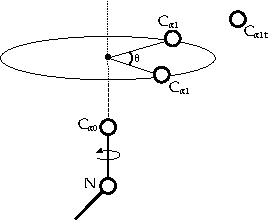
\includegraphics[width=0.75\columnwidth]{figures/ccd_angles}
	\label{fig:ccd_angles}
  \caption{}
\end{figure}



\chapter{Selecting side-chain conformations}
\label{chap:handling_sidechains}
Hvordan vi tilføjer side-chains og derefter tilpasser hele kæden igen.

\section{Related Work}
Todo: snak om SCWRL, der tilføjer side-chains på en fastlåst backbone.



\chapter{Evaluation and results}
To evaluate our solution we have performed experiments on a collection of 100 different proteins.
The average protein length is 78.12 spanning between 11 and 415 amino acids.
The total running time of our fitting algorithm is around 2 minutes for the protein of length 415 on a 1.86GHz CPU (Intel Core 2 Duo, L9400).
There should be ample room for code optimizations as this has not been the focus of the project.

\section{Backbone fitting}
When fitting a protein to a given \Ca-trace we are interested in minimizing the RMSD while avoiding collisions.
In this section we will only consider the RMSD as the evaluation of our collision avoidance method  is postponed until Section \ref{sec:evaluation_handling_side-chains}. 

Typically we are able to reach an RMSD less than 0.2 Å with our backbone fitting algorithm (Algorithm \ref{alg:ccd}).
This is considered satisfactory by the algorithms group at our department.
% We will wait until Sectionwill not consider the collision when evaluating the backbone fitting algorithm.
%In this experiment we have let our algorithm perform the same amount of work for different window sizes (ie. for small $w$ the number of window repetitions is large and vice versa).
%\newpage\vspace*{-15mm}
\subsection{Choice of window size}
As our fitting method performs CCD on a window within the backbone it is interesting to investigate the effect when varying the window size $w$.
Figure \ref{fig:rmsd_convergence} shows the RMSD for four different window sizes $w$ as we repeat the fitting algorithm one to ten times.
\begin{figure}
	\centering
	\hspace*{-3.5mm}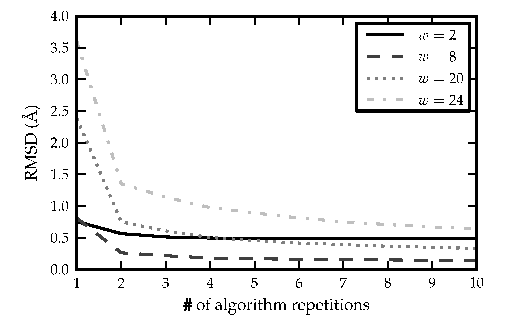
\includegraphics[width=1.1\columnwidth]{figures/plot_rmsd_convergence}
	\caption{RMSD as the fitting progresses for different choices of window size $w$.}
	\label{fig:rmsd_convergence}
\end{figure}
After the first iteration we see that a small window size allows the fitting method to be flexible and reach a low RMSD quickly.
However, if $w$ is too small, the fitting does not improve as we repeat the algorithm.
This is because the chosen angles from a small window are too greedy and find local solutions that lead to an unfavorable global backbone conformation.
On the other hand if $w$ is too large, we see that the RMSD improves in each iteration but requires many iterations to reach a low RMSD.
The problem is caused by the end-effector containing too many elements such that there is no clear direction towards the target since all the elements of the end-effector might go in different directions to reach their separate targets.
This results in small angular changes in each step of the CCD method and a slow RMSD convergence.
Thus, in determining the window size we must strike a balance between small and flexible to get fast convergence and large with the ability to better capture the optimal global solution.
To better illustrate the relationship between RMSD and $w$, the RMSD after 10 repetitions is plotted as a function of $w$ in Figure \ref{fig:rmsd_windowsize}.
We see that the optimal window size is between 5 and 12 amino acids.
\begin{figure}
	\centering
	\hspace*{-3.5mm}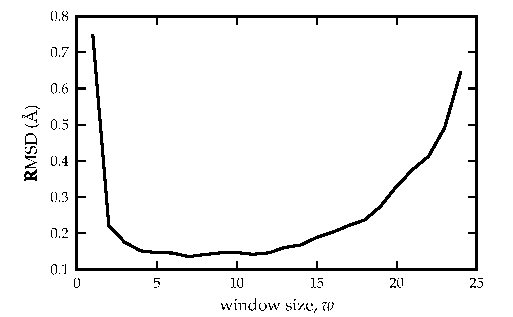
\includegraphics[width=1.1\columnwidth]{figures/plot_rmsd}
	\caption{RMSD as a function of the window size.}
	\label{fig:rmsd_windowsize}
\end{figure}



\subsection{Ramachandran plot}
To check if our fitted backbone structure contains realistic pairs of $\phi$ and $\psi$ angles we can inspect the resulting Ramachandran plots.
Figure \ref{fig:eval_ramachandran} shows two Ramachandran plots of a protein and our fitted backbone version of the same protein.
In the fitted protein, the dense region (the $\alpha$-helix region) resembles the original.
There is also a very slight resemblance in the upper left corner (the $\beta$-sheet region).
For the fitted protein a large part of the angle sets are spread out in the Ramachandran space.
This indicates that we are likely to have unrealistic angle sets since these do not occur in the original backbone nor in Figure \ref{fig:ramachandran}.

\begin{figure*}
	\centering
	\hspace{1cm}\subbottom[]{\hspace{0.2cm}
\includegraphics[width=0.75\columnwidth]{figures/plot_ramachandran_orig}\hspace{1cm} \label{fig:eval_ramachandran_orig}}\hspace{0.5cm}\subbottom[]{\label{fig:eval_ramachandran_fitted}\hspace{0.3cm}
\includegraphics[width=0.75\columnwidth]{figures/plot_ramachandran}\hspace{1cm} }
	\caption{Ramachandran plot of \textbf{(a)} an original protein of length 415 \textbf{(b)} a protein backbone fitted to the original protein (RMSD $=0.15$ Å).}
	\label{fig:eval_ramachandran}
\end{figure*}


\section{Collision handling}
To count the number of collisions we employ a simple collision detection method that for all atom pairs (except for bonded pairs) checks whether the two atoms are within a certain distance of each other.
A more realistic collision detection method utilizes different atom radii depending on the atom types \cite{bondi1964van}. 
This is beyond the scope of the project.

Since not all proteins in our collection contain hydrogen atoms (these are omitted if the resolution of the X-ray crystallography used to determine the protein structure is too low), we ignore all hydrogen atoms when counting collisions.
Instead, we have increased the collision distance accordingly.
The collision distance we used in the following is 1.25 Å.

\subsection{Collision handling with fitted backbones}
After having fitted the protein backbone to a \Ca-trace, the side-chain rotamers are chosen as described in Section \ref{chap:handling_sidechains} such that the number of collisions is minimized.
There is a correlation between the average number of collisions in a fitted protein and how well we are able to fit it to the backbone. 
For small RMSDs (less than 0.1 Å), the number of collisions is around 1 every 100 amino acids before our side-chain positioning (SCP) algorithm.
After SCP, the number of collisions is brought down to 1 every 500 amino acids.
	%Thus, collisions are more likely to occur in large proteins.

In Figure \ref{fig:plot_scp} we have plotted the average number of collisions after SCP as a function of the number of initial collisions.
In our experience, the collision avoidance algorithm is working quite efficiently reducing the number of collisions in a protein by a factor of ten on average. \fixme{det er snarere en faktor 7 (skal også fikses i abstract)}
We have performed a visual inspection on the remaining collisions and the majority of the collisions is caused by either: 
1. A proline amino acid is given an unfavorable set of $\phi$ and $\psi$ angles such that the backbone will collide with all of the proline rotamers.
2. The backbone is folded unfavorably such that the amino acids are placed too close making side-chain collisions inevitable.
Thus, both problems are caused by a deficient fitting algorithm.

Varying the search depth parameter for the SCP algorithm has little effect for depths over 3.
When the search depth is below 3 we see that the number of resolved collisions drops.

\label{sec:evaluation_handling_side-chains}
\begin{figure}
	\centering
	\hspace*{-3.5mm}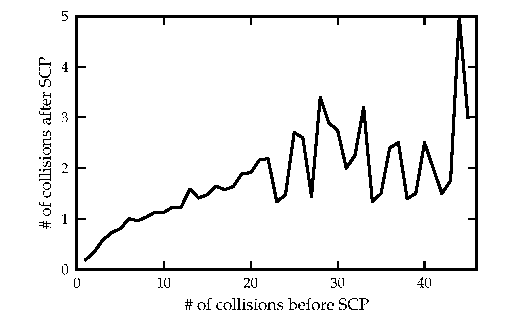
\includegraphics[width=1.1\columnwidth]{figures/plot_scp}
	\caption{SCP performance: The average number of collisions as a function of the number of initial collision. The fluctuations in the right half of the plot is caused by noise.}
	\label{fig:plot_scp}
\end{figure}

\subsection{Collision handling with realistic backbones}
To verify our claim that the collisions are caused by an unfavorable backbone folding, we have performed SCP on a collection of realistic backbones generated by X-ray crystallography.
That is, we are only adjusting side-chain conformations on protein backbones extracted from \url{http://www.pdb.org}. 

With realistic backbone, we get significantly better results.
In a collections of 383 proteins with an average length of 215 amino acids, we have approximately 1 collision every 7500 amino acids after SCP.
A visual inspection reveals that the remaining collisions are caused by the rotamer library not being flexible enough since these collisions could be avoided by small modifications of the $\chi$ angles.


\section{Comparison with SCWRL}

%%% Local Variables: 
%%% mode: latex
%%% TeX-master: "rapport"
%%% End: 


\chapter{Future Work}
Use probability maps to accept or reject $\phi$ and $\psi$ angles proposed by the CCD-algorithm.

Some method\texttrademark\ to detect when backbone is folded making side-chain collisions inevitable

Experiment with $\omega$ angles. They should not be adjusted by the CCD method in each iteration (too expensive) but be tested if we get a bad fit in a small amino acid subsequence.

\section{Experiment with Hydrogen atoms}
How large is the variability of the hydrogen atoms in the backbone and
side-chains? How hard would it be to add hydrogen atoms on to an
otherwise full model of the protein? If the hydrogen atoms are easy to
add later, we could post-pone the problem of adding them and thereby
simplifying our model.


%%% Local Variables: 
%%% mode: latex
%%% TeX-master: "rapport"
%%% End: 


\chapter{Conclusion}
In this report we have investigated a strategy for predicting the native structure of proteins including all atoms from an already folded $C_\alpha$-trace as target. 
We have decomposed the problem into two separate subtasks:
Fitting the all-atom backbone to the given \Ca-trace and selecting side-chain rotamers while minimizing the number of collisions.

We have devised our own variant of the CCD method to solve the inverse kinematics problem of fitting the backbone structure to the given \Ca-trace. 
Typically we are able to reach an RMSD less than 0.2 Å.

For the problem of positioning side-chains on the backbone and
selecting side-chain conformations with few or no collisions, we use
a simple algorithm that iteratively goes through the amino acid trying
to eliminate eventual collisions one at a time. We have experienced reductions in the number of collision in proteins by an average factor of ten.




%\defbibheading{bibliography}[\bibname]{
% \chapter{#1}
% \markboth{#1}{#1}}
\defbibheading{bibliography}{\chapter{Bibliography}} 
\printbibliography

\end{document}

